\begin{strip}
\centering
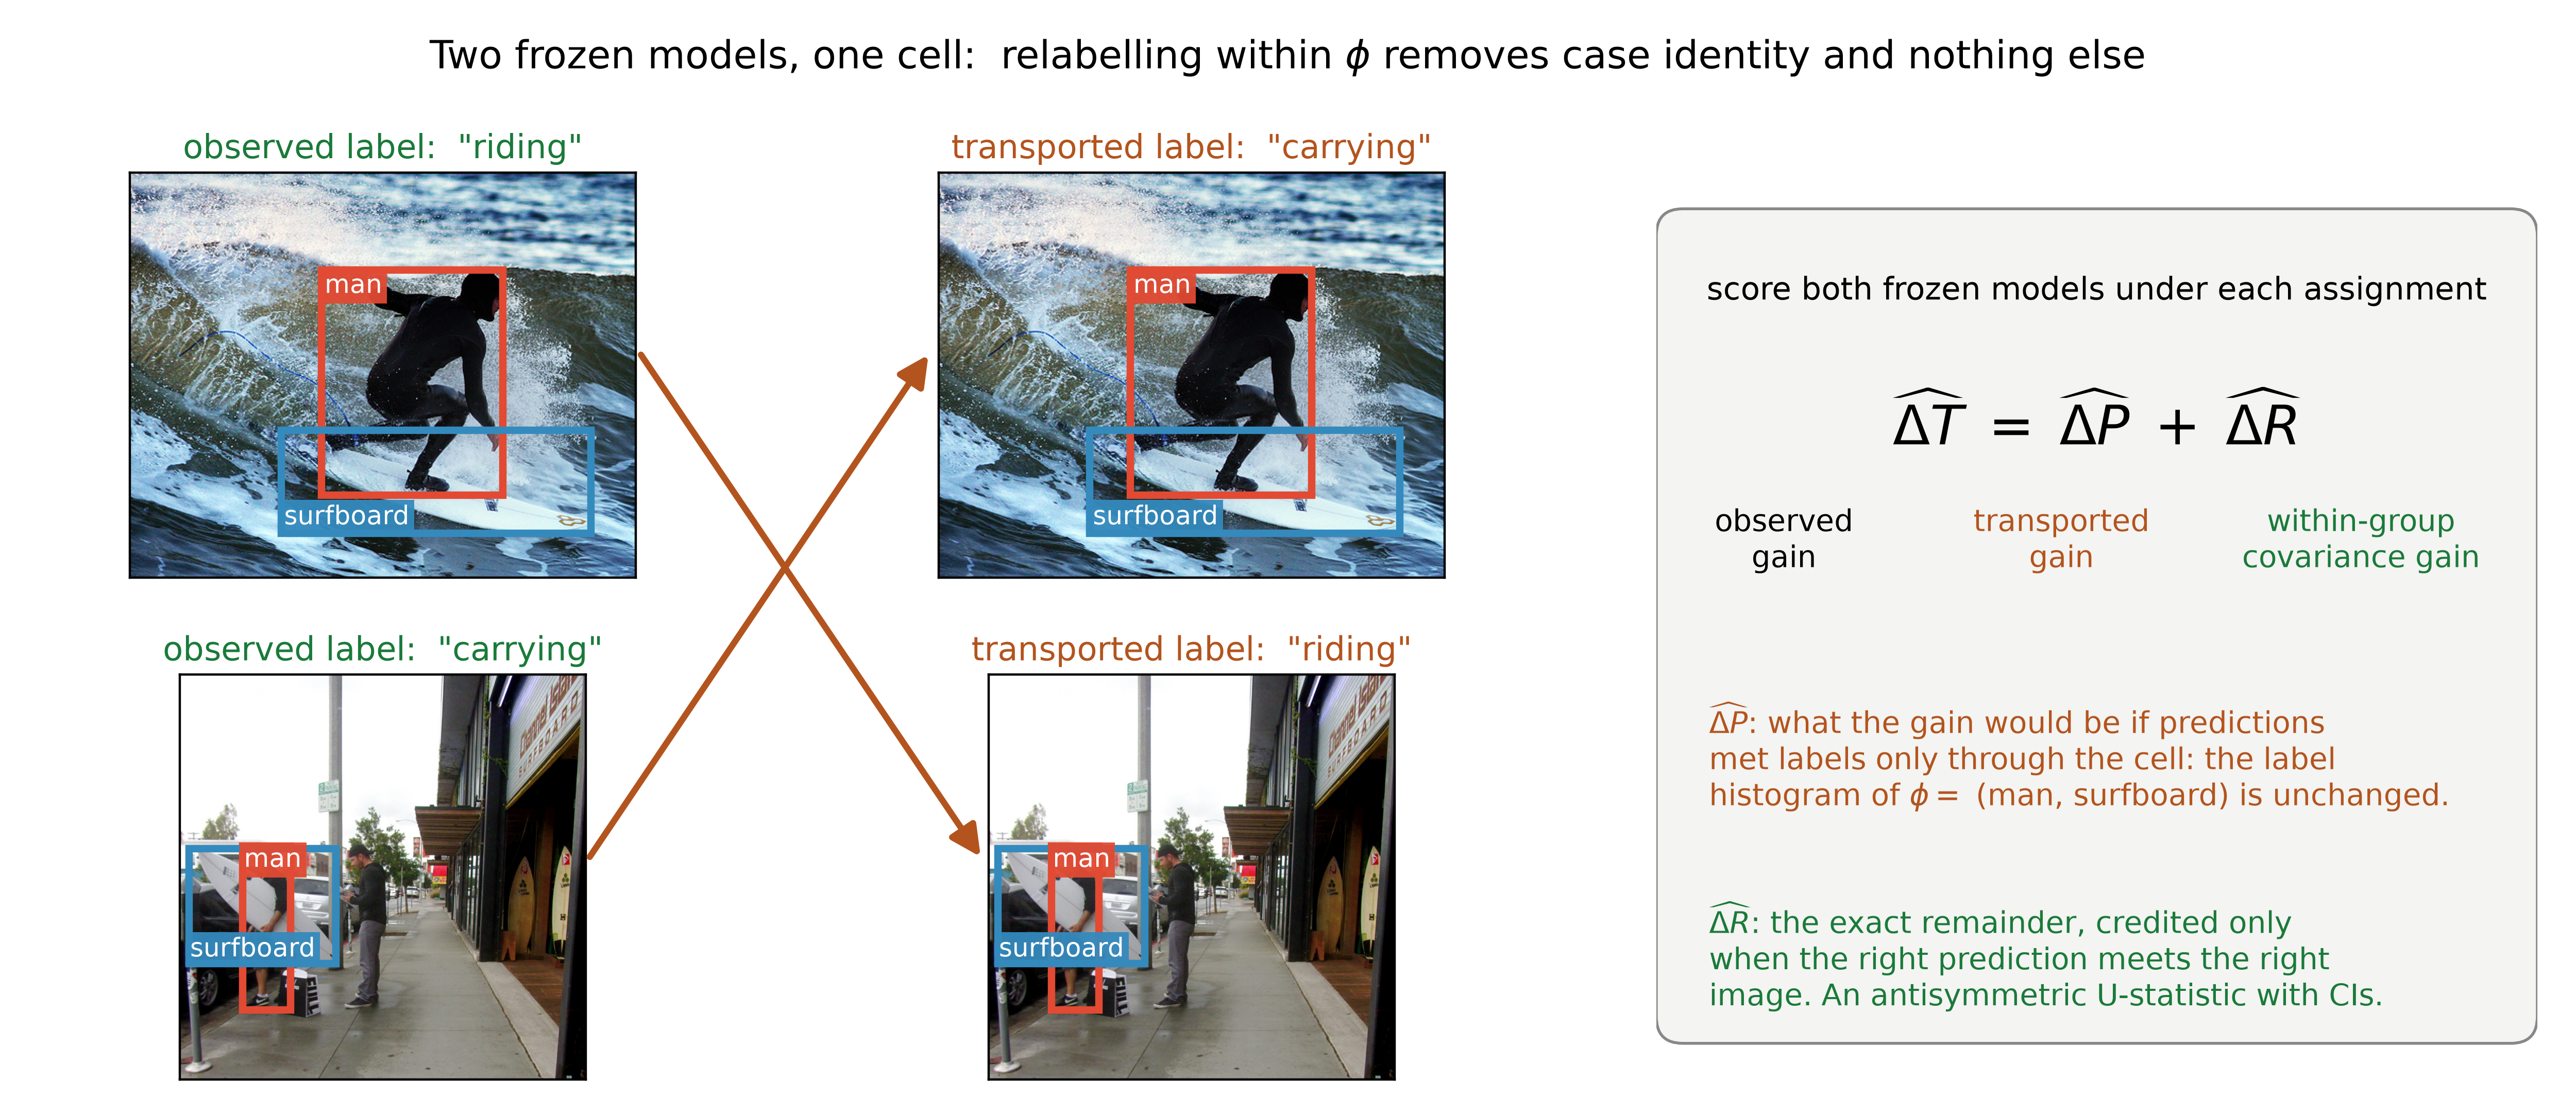
\includegraphics[width=\linewidth]{figures/fig1_new_concept.png}
\captionsetup{hypcap=false}
\captionof{figure}{\textbf{Within-group relabelling.} Two Visual Genome relations share the
subject--object pair (\textsf{man}, \textsf{surfboard}). Swapping their labels keeps the
pair's predicate histogram exactly as it was but breaks the link between each image and its
own label. Scoring two frozen models under the observed and the swapped labels splits
their score gain exactly: $\hdP$ is the part that survives the swap --- earned at the level
of the group --- and $\hdR$ is the covariance between each relation's prediction and its own
label, which better ranking within the group can supply, and so can a moved operating point.}
\captionsetup{hypcap=true}
\label{fig:concept}
\end{strip}
